\section{Execução e Validação Experimental}
\label{sec:validacao}

Os experimentos foram conduzidos em uma estação host Linux Ubuntu 24.04.4 LTS (kernel \texttt{6.14.0-33-generic}, \texttt{x86\_64}) executando o cluster Minikube \texttt{v1.39.0} (Kubernetes \texttt{v1.37.0}, runtime \texttt{containerd 2.3.4} e plugin CNI Calico). Os ensaios de autorrecuperação, escala e persistência foram repetidos em $n = 5$ rodadas. Os resultados estão na Tabela~\ref{tab:resultados-experimentais}.

\begin{table*}[t]
\centering
\caption{Resultados Quantitativos dos Ensaios de Autorrecuperação, Escalabilidade Horizontal e Persistência Transacional ($n = 5$)}
\label{tab:resultados-experimentais}
\scriptsize
\setlength{\tabcolsep}{1.8pt}
\begin{tabular*}{\textwidth}{@{\extracolsep{\fill}}c cccc c cccc@{}}
\toprule
 & \multicolumn{4}{c}{\textbf{1. Autorrecuperação de Pod (\texttt{selfheal.csv})}} & \multicolumn{1}{c}{\textbf{2. Escala (\texttt{scale.csv})}} & \multicolumn{4}{c}{\textbf{3. Persistência no PostgreSQL (\texttt{persistencia.csv})}} \\
\cmidrule(lr){2-5} \cmidrule(lr){6-6} \cmidrule(l){7-10}
\textbf{Rodada} & \textbf{\texttt{3/3 Ready} (s)} & \textbf{Erros} & \textbf{Reqs.} & \textbf{Sucesso (\%)} & \textbf{\texttt{3$\rightarrow$10 Ready} (s)} & \textbf{Antes} & \textbf{Depois} & \textbf{$\Delta$} & \textbf{Retenção} \\
\midrule
1 & 5,96 & 0 & 34 & 100,00\% & 7,16 & 314 & 315 & $+1$ & 100\% (0 perda) \\
2 & 5,84 & 1 & 34 & 97,06\%  & 6,58 & 260 & 261 & $+1$ & 100\% (0 perda) \\
3 & 8,84 & 0 & 40 & 100,00\% & 6,82 & 282 & 283 & $+1$ & 100\% (0 perda) \\
4 & 8,83 & 0 & 37 & 100,00\% & 6,80 & 502 & 503 & $+1$ & 100\% (0 perda) \\
5 & 8,38 & 0 & 37 & 100,00\% & 6,75 & 524 & 525 & $+1$ & 100\% (0 perda) \\
\midrule
\textbf{Média $\pm$ DP} & $\mathbf{7{,}57 \pm 1{,}54\,\textbf{s}}$ & $\mathbf{0{,}20 \pm 0{,}45}$ & $\mathbf{36{,}40 \pm 2{,}51}$ & $\mathbf{99{,}45\%\ (181/182)}$ & $\mathbf{6{,}82 \pm 0{,}21\,\textbf{s}}$ & --- & --- & $\mathbf{+1{,}00 \pm 0{,}00}$ & $\mathbf{100\%\ (5/5)}$ \\
\bottomrule
\end{tabular*}
\end{table*}

\subsection{Balanceamento de Carga e Exposição via NodePort}
A validação do plano de dados em regime nominal iniciou-se com a inspeção das 3 réplicas do \texttt{Deployment api} (\texttt{api-58cf7fff8c-8kbgh}, \texttt{b5mqd} e \texttt{qtbx5}), alocadas na sub-rede \texttt{10.244.120.70}--\texttt{72} e vinculadas ao objeto \texttt{Endpoints} do serviço \texttt{api} (\texttt{NodePort 10.99.68.112}, mapeamento \texttt{80:30080/TCP}). Em razão do encerramento explícito de conexões TCP a cada resposta (\texttt{Connection: close} e \texttt{keepalive = 0}), uma sequência de 20 requisições consecutivas a \texttt{/api/whoami} (\texttt{relatorio/logs/17-r4.txt}) demonstrou alternância efetiva entre os três backends pelas regras \texttt{iptables} do \texttt{kube-proxy}, enquanto o contador transacional \texttt{visits} progrediu monotonamente de \texttt{21} a \texttt{40}:

\begin{lstlisting}
NAME  TYPE      CLUSTER-IP    PORT(S)       AGE
api   NodePort  10.99.68.112  80:30080/TCP  85s
NAME  ENDPOINTS
api   10.244.120.70:8080,10.244.120.71:8080,
      10.244.120.72:8080
# Sequencia de respostas (pod / db / visits):
api-58cf7fff8c-b5mqd   ok   23
api-58cf7fff8c-8kbgh   ok   24
api-58cf7fff8c-b5mqd   ok   25
api-58cf7fff8c-8kbgh   ok   28
api-58cf7fff8c-qtbx5   ok   31
api-58cf7fff8c-qtbx5   ok   39
\end{lstlisting}

A Figura~\ref{fig:r4-pagina} apresenta a interface web de monitoramento servida pela aplicação durante o teste, evidenciando a detecção simultânea das três réplicas (\texttt{8kbgh}, \texttt{b5mqd} e \texttt{qtbx5}), latência média de $16\,\text{ms}$, ausência de falhas HTTP e distribuição equilibrada na barra histórica das últimas 40 respostas.

\begin{figure}[t]
\centering
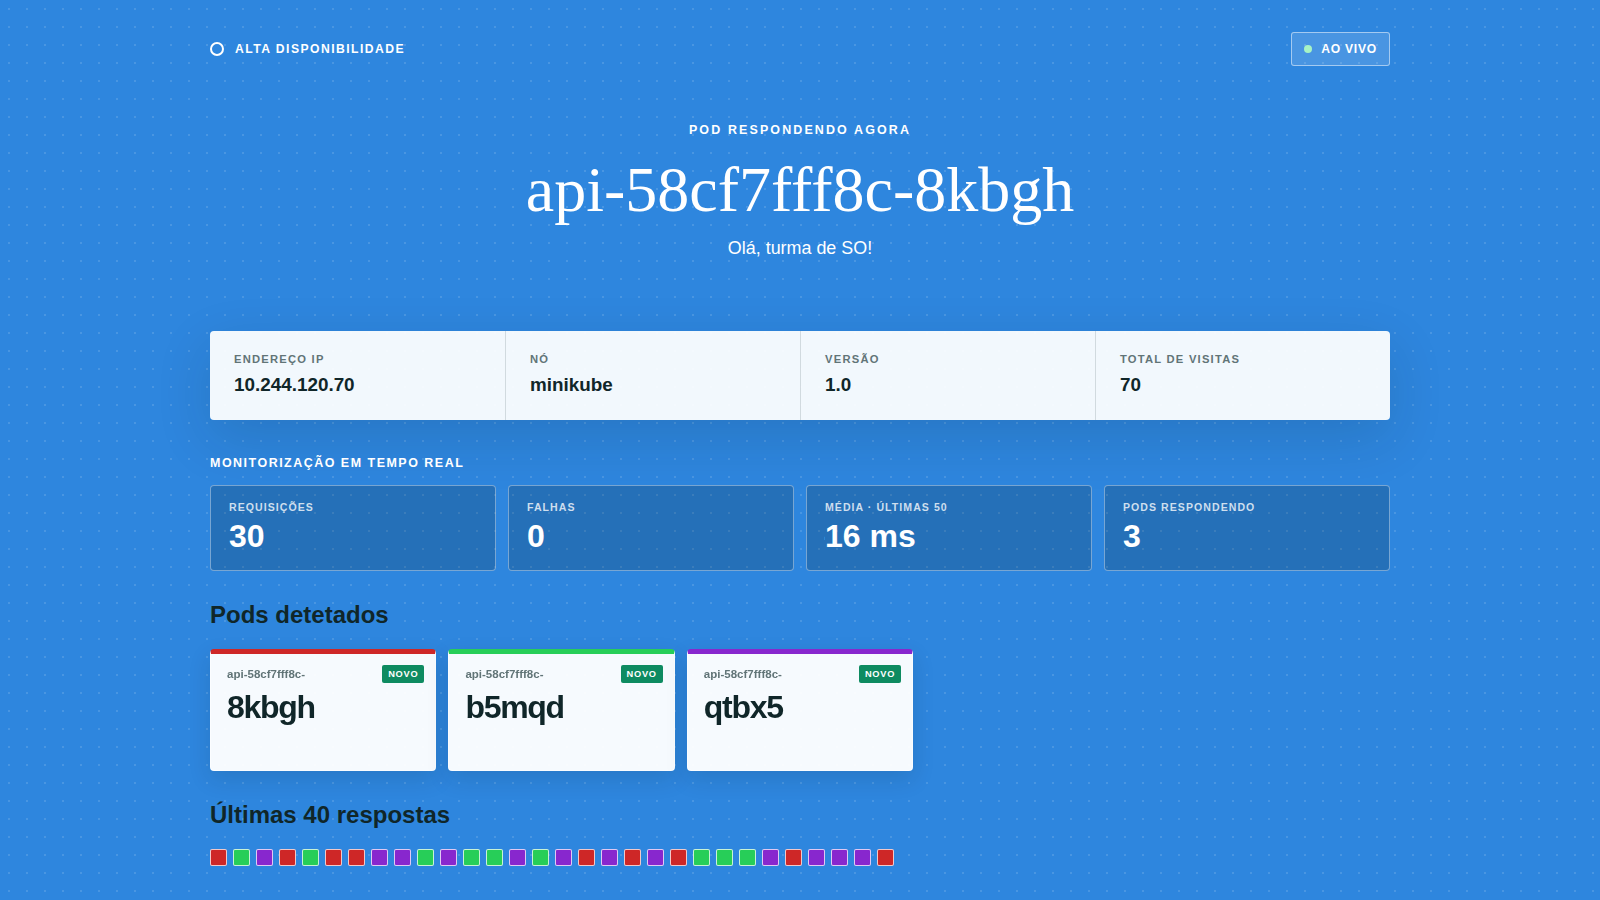
\includegraphics[width=0.84\columnwidth]{figuras/17-r4-pagina.png}
\caption{Painel de telemetria em operação nominal com 3 réplicas ativas (\texttt{8kbgh}, \texttt{b5mqd} e \texttt{qtbx5}), latência média de $16\,\text{ms}$ e balanceamento de carga L4 entre os pods.}
\label{fig:r4-pagina}
\end{figure}

\subsection{Autorrecuperação (\textit{Self-Healing}) de Pods e de Processo}
A resiliência da camada de aplicação foi avaliada sob duas modalidades de injeção de falhas:
\begin{enumerate}
    \item \textbf{Remoção abrupta de pod (\texttt{kubectl delete pod}):} A exclusão da réplica \texttt{api-58cf7fff8c-8kbgh} (\texttt{UID 3464f481-...}) sensibilizou imediatamente o laço de reconciliação do controlador \texttt{ReplicaSet} no \texttt{kube-controller-manager}. Ao detectar a divergência entre \texttt{spec.replicas: 3} e apenas 2 réplicas ativas, o controlador emitiu o evento \texttt{SuccessfulCreate} para o pod substituto \texttt{api-58cf7fff8c-wbgrv} (\texttt{IP 10.244.120.77}) no mesmo segundo em que o pod original entrou em estado \texttt{Killing}/\texttt{Terminating}, restabelecendo a condição \texttt{3/3 Ready} em $5897\,\text{ms}$. A Figura~\ref{fig:r5-transicao} ilustra, via \texttt{kubectl get pods -n ha-demo -w}, a transição completa de estados no kernel e no runtime (\texttt{Terminating} $\rightarrow$ \texttt{Pending} $\rightarrow$ \texttt{Init:0/1} $\rightarrow$ \texttt{PodInitializing} $\rightarrow$ \texttt{Running 1/1} em $5\,\text{s}$ na réplica substituta \texttt{9xwwk}). Nas $n = 5$ execuções automatizadas com sondagem HTTP a cada $100\,\text{ms}$ (Tabela~\ref{tab:resultados-experimentais}), o tempo médio de convergência até \texttt{3/3 Ready} foi de $7{,}57 \pm 1{,}54\,\text{s}$, com taxa global de disponibilidade HTTP de $99{,}45\%$ ($181/182$ requisições bem-sucedidas, registrando-se um único erro transitório na Rodada 2 durante a janela sub-segundo de atualização das regras \texttt{iptables}).
    \item \textbf{Travamento lógico de processo (\texttt{POST /api/crash}):} A criação do arquivo sentinela \texttt{/tmp/unhealthy} faz com que a rota \texttt{GET /healthz} passe a retornar HTTP \texttt{500}. Após \texttt{failureThreshold: 3} verificações consecutivas da \texttt{livenessProbe} (\texttt{periodSeconds: 5}, totalizando $\approx 15\,\text{s}$), o agente \texttt{kubelet} reinicia o container \texttt{api} in-loco, incrementando o contador \texttt{RESTARTS} sem alterar o \texttt{POD\_NAME} ou o \texttt{POD\_IP} e limpando o sistema de arquivos efêmero do container.
\end{enumerate}

\begin{figure}[t]
\centering
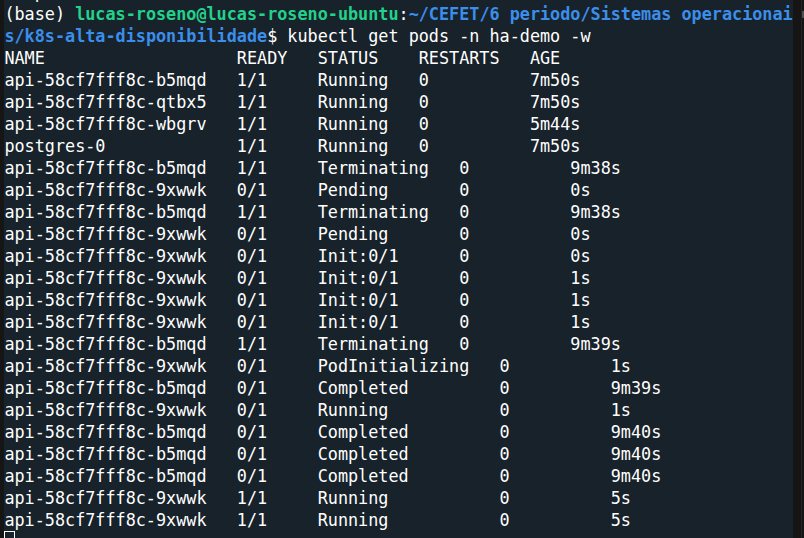
\includegraphics[width=0.84\columnwidth]{figuras/17-r5-transicao.png}
\caption{Captura em tempo real (\texttt{kubectl get pods -n ha-demo -w}) do ciclo de autorrecuperação: transição \texttt{Terminating} $\rightarrow$ \texttt{Pending} $\rightarrow$ \texttt{Init:0/1} $\rightarrow$ \texttt{PodInitializing} $\rightarrow$ \texttt{Running 1/1} em $5\,\text{s}$.}
\label{fig:r5-transicao}
\end{figure}

\subsection{Elasticidade Horizontal Imperativa ($3 \rightarrow 10$ Réplicas) e Reativa (\texttt{HPA})}
\begin{itemize}
    \item \textbf{Escalonamento Imperativo e Teste de Estresse Concorrente:} O disparo de \texttt{kubectl scale deployment api -n ha-demo -{}-replicas=10} instanciou 7 novas réplicas (\texttt{96rnn}, \texttt{9d74k}, \texttt{cggt4}, \texttt{j9hk2}, \texttt{k2fcw}, \texttt{kxzrl} e \texttt{qwrrm}, IPs \texttt{10.244.120.78}--\texttt{84}), atingindo \texttt{10/10 Ready} em $6{,}82 \pm 0{,}21\,\text{s}$ na média das 5 execuções (Tabela~\ref{tab:resultados-experimentais}). O baixo desvio-padrão decorre da retenção local das imagens OCI no \texttt{containerd} e da prontidão imediata do serviço \texttt{postgres} no \texttt{initContainer}. A Figura~\ref{fig:r6-dez-pods} exibe o painel web com os 10 pods respondendo simultaneamente e latência média reduzida para $13\,\text{ms}$. Submetido a uma bateria de estresse de $3000$ requisições concorrentes (20 clientes paralelos via \texttt{xargs -P 20}), o conjunto de 10 réplicas (40 \textit{threads} Gunicorn) processou $100\%$ das chamadas ($3000/3000$) com \texttt{\textquotedbl{}db\textquotedbl{}:\textquotedbl{}ok\textquotedbl{}}, enquanto o pod \texttt{postgres-0} operou em $172\,\text{mCPU}$ e $39\,\text{MiB}$ de RAM, abaixo dos seus limites de \texttt{cgroups} (\texttt{250m}/\texttt{512Mi}).
    \item \textbf{Autoescalonamento Reativo via \texttt{HPA}:} Em repouso, \texttt{kubectl top pods} indicou consumo de $2\,\text{mCPU}$ e $76\,\text{MiB}$ por réplica da API (\texttt{TARGETS: cpu: 2\%/50\%}). Com a ativação do gerador de carga \texttt{scripts/load-hpa.sh} (6 fluxos concorrentes em \texttt{/api/cpu?ms=200}), a utilização média subiu a $230\%$ do \texttt{request} ($113\text{--}143\,\text{mCPU}$ por pod), levando o \texttt{HPA} a expandir o \texttt{Deployment} progressivamente de $3 \rightarrow 6 \rightarrow 10$ réplicas em $30\,\text{s}$, diluindo a carga média para $133\%$ (\texttt{4m45s}):
\end{itemize}

\begin{lstlisting}
$ kubectl get hpa -n ha-demo -w
NAME REFERENCE      TARGETS       MIN MAX REPLICAS AGE
api  Deployment/api cpu: 2%/50%   3   10  3        80s
api  Deployment/api cpu: 230%/50% 3   10  3        2m45s
api  Deployment/api cpu: 230%/50% 3   10  6        3m
api  Deployment/api cpu: 230%/50% 3   10  10       3m15s
api  Deployment/api cpu: 133%/50% 3   10  10       4m45s
# Apos encerrar carga (estabilizacao de 300s):
api  Deployment/api cpu: 2%/50%   3   10  10       31m
api  Deployment/api cpu: 2%/50%   3   10  3        35m
\end{lstlisting}

\begin{figure}[t]
\centering
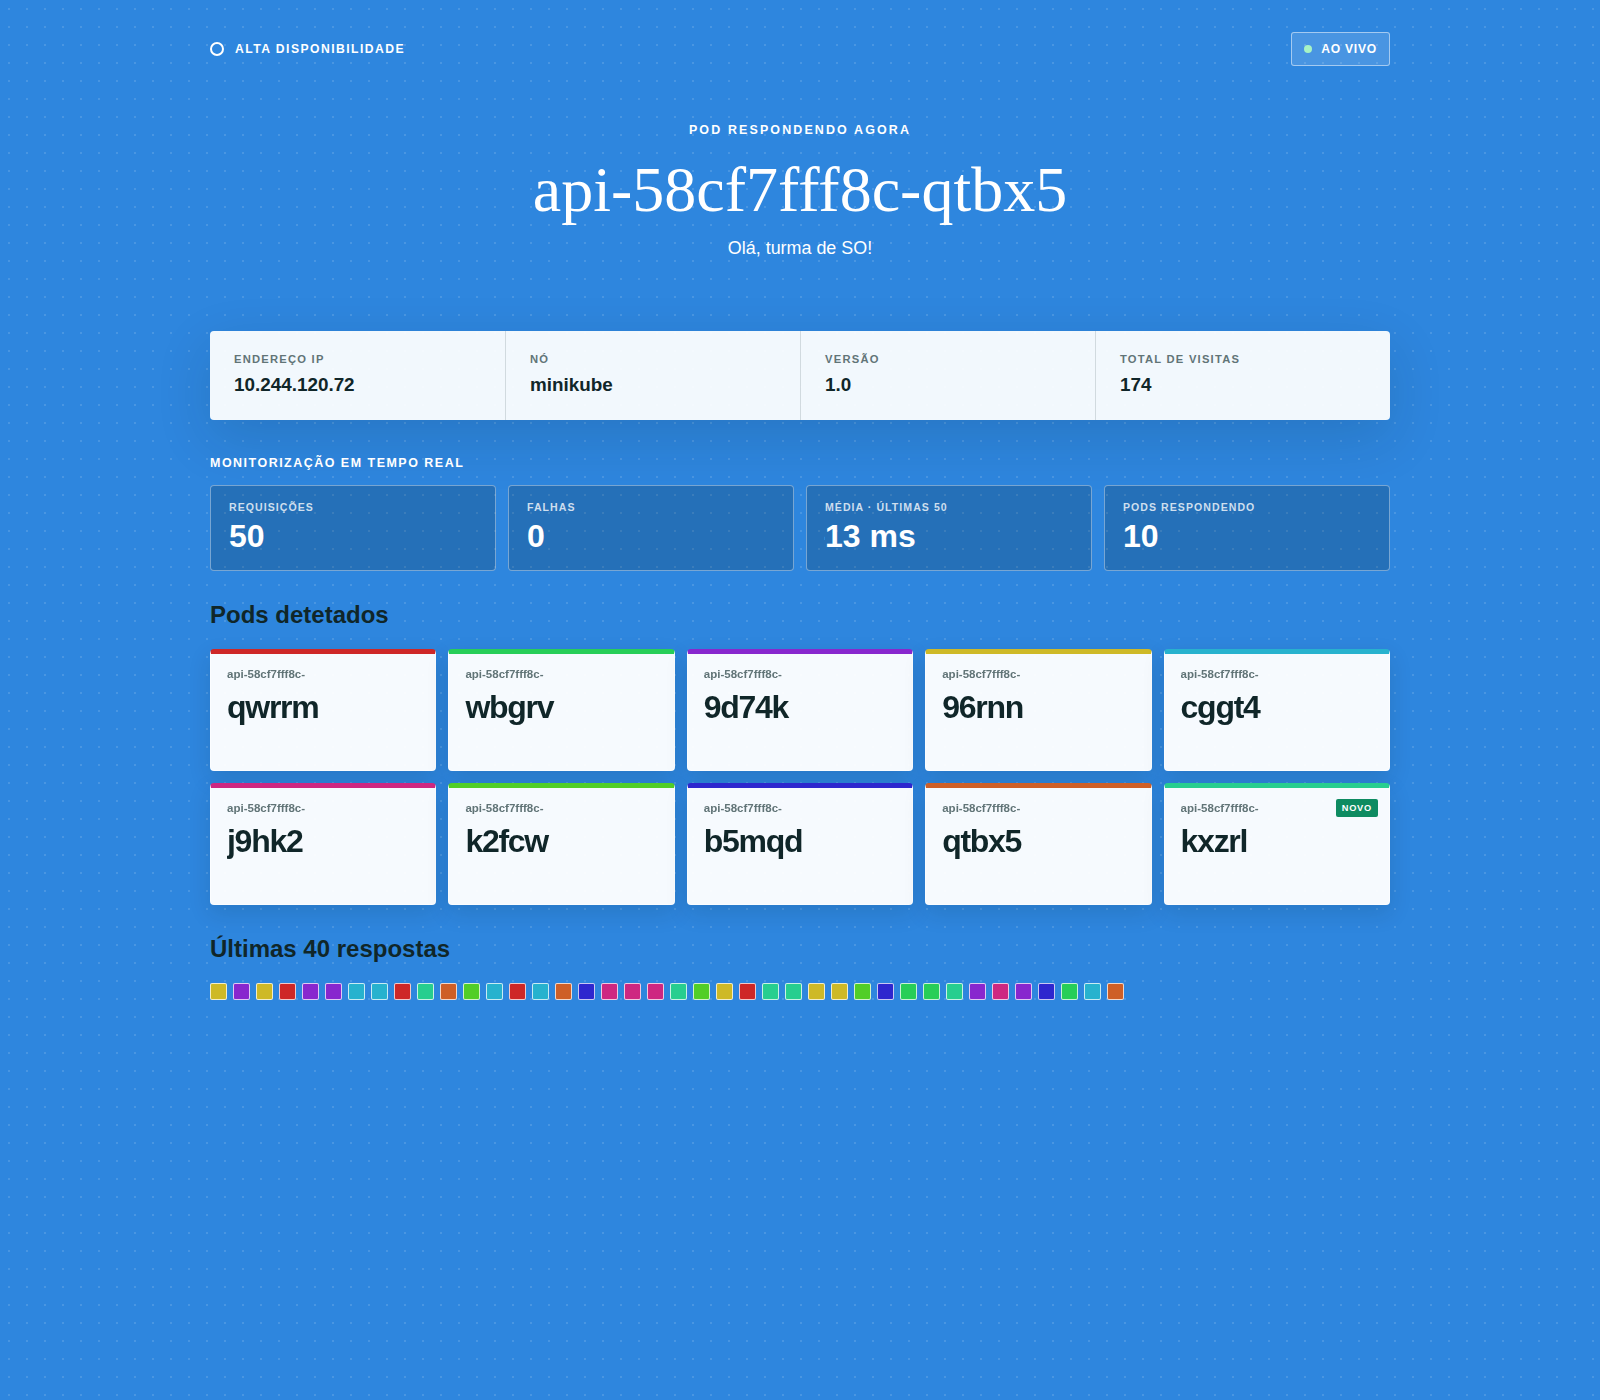
\includegraphics[width=0.84\columnwidth]{figuras/17-r6-dez-pods.png}
\caption{Painel web após escalonamento horizontal para 10 réplicas ativas no namespace \texttt{ha-demo}, operando com zero falhas e latência média de $13\,\text{ms}$.}
\label{fig:r6-dez-pods}
\end{figure}

\subsection{Persistência Transacional, Degradação Graciosa, Isolamento de Rede e Operação Offline}
\begin{itemize}
    \item \textbf{Persistência em \texttt{StatefulSet}/\texttt{PVC} e Degradação Graciosa:} Na Rodada 1 da Tabela~\ref{tab:resultados-experimentais}, após acumular \texttt{visits: 314}, o pod \texttt{postgres-0} foi removido (\texttt{kubectl delete pod postgres-0 -n ha-demo}). Durante os $7\,\text{s}$ de recriação do container pelo \texttt{StatefulSet}, chamadas a \texttt{/api/whoami} retornaram \texttt{HTTP/1.1 200 OK} com payload degradado (\texttt{\textquotedbl{}visits\textquotedbl{}:null, \textquotedbl{}db\textquotedbl{}:\textquotedbl{}indisponível\textquotedbl{}}). Graças ao desacoplamento da sonda \texttt{GET /readyz}, as 3 réplicas da API permaneceram ativas no \texttt{Service}, e o painel web (Figura~\ref{fig:painel-banco-fora}) exibiu o alerta \textquotedbl{}BANCO FORA DO AR\textquotedbl{} preservando em tela a última contagem válida sem erros HTTP. Concluída a prontidão do novo \texttt{postgres-0}, o volume \texttt{data-postgres-0} manteve exatamente o mesmo identificador (\texttt{UID 873f564d-32f8-4e88-8472-cb408247b7b9}) e a requisição seguinte registrou \texttt{visits: 315} (\texttt{\textquotedbl{}db\textquotedbl{}:\textquotedbl{}ok\textquotedbl{}}), comprovando retenção integral do estado em todas as 5 execuções ($\Delta = +1$).
    \item \textbf{Isolamento de Rede via Calico \texttt{NetworkPolicy}:} Com a política \texttt{postgres-allow-api} ativa, um pod efêmero sem o rótulo autorizado (\texttt{kubectl run intruso -{}-image=busybox:1.36}) teve pacotes SYN descartados pelo \textit{netfilter} ao testar a porta \texttt{5432} (\texttt{nc: postgres (10.244.54.229:5432): Connection timed out}, código de saída \texttt{1}), enquanto um pod rotulado com \texttt{app=api} (\texttt{amigo}) estabeleceu conexão TCP imediata (\texttt{postgres (10.244.54.229:5432) open}, saída \texttt{0}).
    \item \textbf{Atualização Contínua (\textit{Rolling Update}) e Operação 100\% Offline:} A substituição gradual de versão na API sob \texttt{maxSurge: 1} e \texttt{maxUnavailable: 0} manteve 100\% de disponibilidade durante a transição. Por fim, bloqueando-se todo o tráfego externo de internet no nó Minikube via regras \texttt{iptables REJECT} nas cadeias \texttt{OUTPUT} e \texttt{FORWARD} (confirmado pela falha de conexão a \texttt{https://registry-1.docker.io/v2/}), a recriação completa do ambiente (\texttt{reset.sh} + \texttt{deploy.sh}) e a exclusão forçada do \texttt{postgres-0} convergiram para \texttt{Running 1/1} em $6\text{--}12\,\text{s}$ com eventos \texttt{Pulled: Container image already present on machine}, validando a autonomia offline proporcionada por \texttt{imagePullPolicy: IfNotPresent}.
\end{itemize}

\begin{figure}[t]
\centering
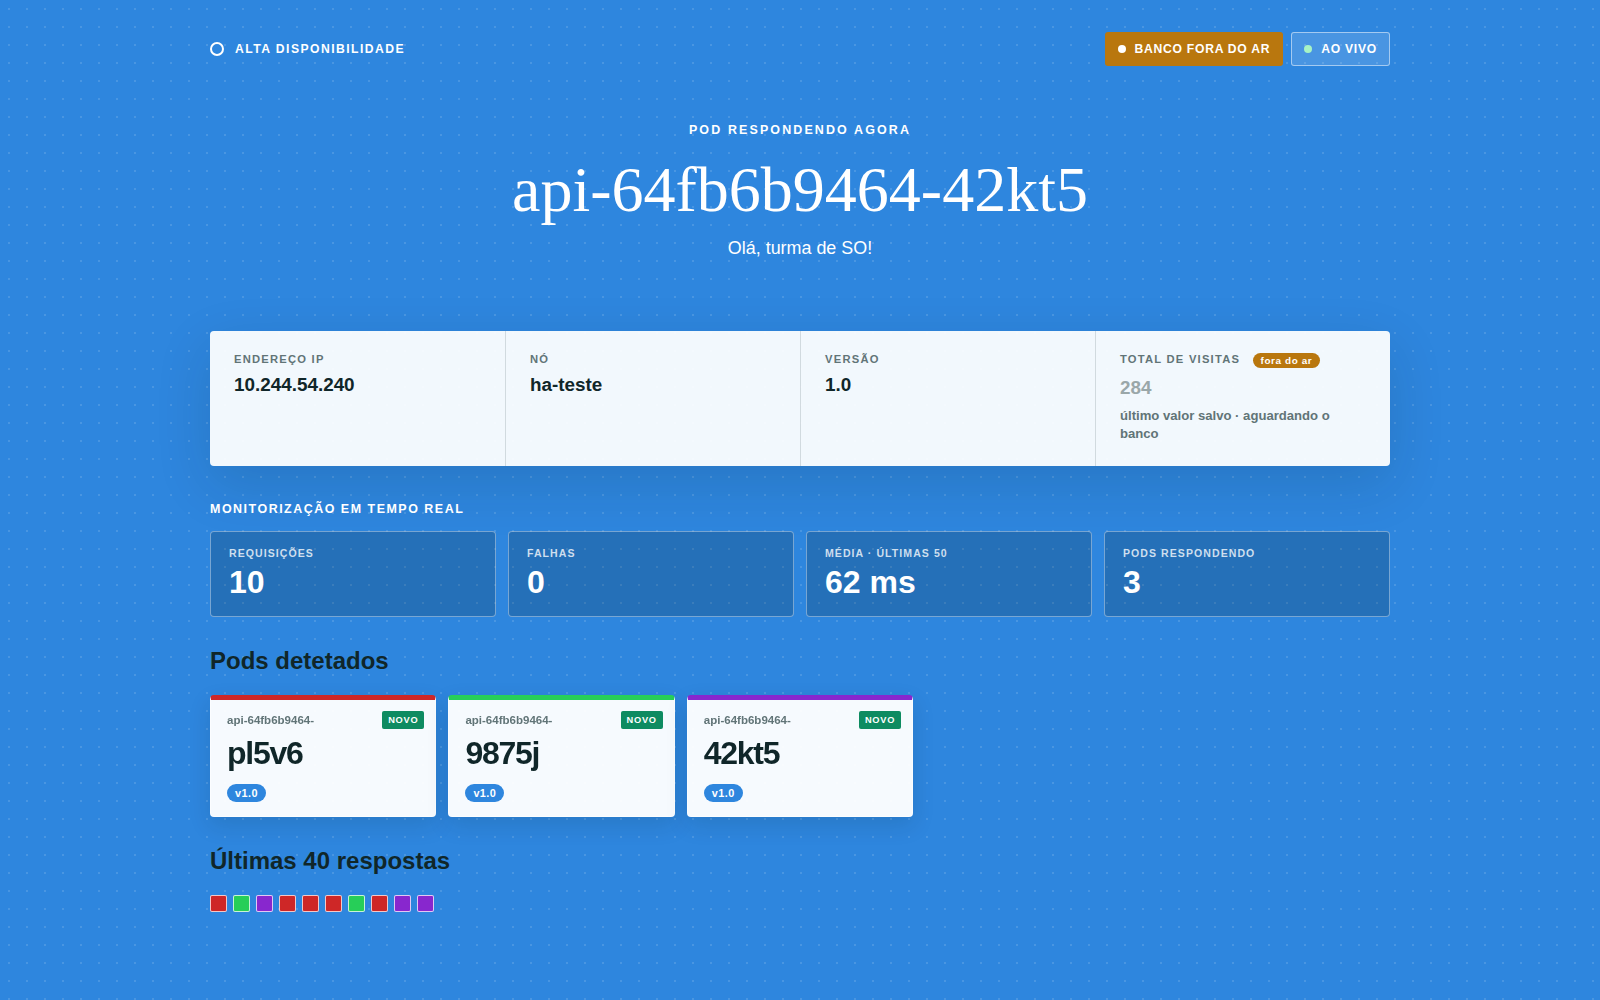
\includegraphics[width=0.84\columnwidth]{figuras/22-painel-banco-fora.png}
\caption{Degradação graciosa no painel de telemetria durante a recriação do pod \texttt{postgres-0}: sinalização \textquotedbl{}BANCO FORA DO AR\textquotedbl{}, preservação do último contador em cache (\texttt{284}) e zero falhas HTTP nas 3 réplicas da API.}
\label{fig:painel-banco-fora}
\end{figure}
